
\newpage
\section{Mathematical Background*}%
\label{sec:background_}

\subsection{Hilbert Spaces}%
\label{ssub:hilbert_spaces}

We will in this report assume $\Omega $ to be a compact and open set in $\mathbb{R} ^{2}$. Now let the parameter $p \in \mathbb{R} $, $p\ge 1$. We then define the space $L^{p}\left( \Omega  \right) $ to be the set of all measurable functions $f: \Omega  \mapsto \mathbb{R} $ such that
$\left\lvert f \right\rvert ^{p}$ is Lebesgue measurable, i.e,

\begin{equation*}
    L^{p}\left( \Omega  \right) = \left\{ f: \Omega \mapsto \mathbb{R}  \mid \int_{\Omega }^{} \left\lvert f \right\rvert ^{p} d \Omega  < \infty  \right\}
.\end{equation*}

A useful extension, which we will use later, are the set of locally integrable functions for any compact subset $K \subseteq \text{Interior}\left( \Omega  \right) $ \cite{brenner07math}, that is,

\begin{equation*}
    L_{loc}^{1}\left( \Omega  \right)  = \left\{ f: f \in L^{1}\left( \Omega  \right)  \quad \forall K  \right\}.
\end{equation*}
Let $u \in L^{p}\left( \Omega  \right) $. We define the integral norm of order $p$ to be \[
\| u \|_{ L^{p}\left( \Omega  \right)  }^{  }  = \left( \int_{\Omega }^{} \left\lvert u \right\rvert ^{p} dx  \right) ^{\frac{1}{p}}.
\]
Since $p=2$ is frequently used in this report, we also define for convenience a compact notation $\| u \|_{ \Omega  }^{  }  = \| u \|_{ L^{2}\left( \Omega  \right)  }^{  } $ .  We say that $L^{2}\left( \Omega  \right) $ is a Hilbert space if it is equipped with a inner
product of two functions $u,v \in L^{2}\left( \Omega  \right) $ such that
\[
\left( u,v \right) _{\Omega } = \left( u,v \right) _{L^2\left( \Omega  \right) } = \int_{\Omega }^{} u  v dx.
\]

To generalize, we denote the notation $\mathcal{V} $ for a arbitrary Hilbert space. Furthermore, we define the dual space the be the space of linear and bounded functionals $F: \mathcal{V}  \mapsto \mathbb{R} $\cite{quartdiff}, i.e., \[
\mathcal{V} ^{*} =
\left.
\begin{cases}
F: \mathcal{V}  \mapsto \mathbb{R} \text{ such that }\forall v,w \in \mathcal{V}, \forall a,b \in \mathbb{R} \text{ and } C> 0 \text{ is }   \\
  F\left( \lambda v + \mu w  \right) = \lambda F(v) + \mu F(w) \text{ and } \left\lvert F\left( v \right)  \right\rvert \le C \| v \|_{ \mathcal{V}  }^{  }
\end{cases}
  \right\}
\]
and we equip it with the functional norm,  \[
    \| F \|_{ \mathcal{V} ^{*} }^{  } = \sup_{v \in \mathcal{V}   } \frac{\left\lvert F\left( v \right)  \right\rvert }{\| v \|_{ \mathcal{V}  }^{  } }.
\]

We will now establish a notion of the weak derivative, but first are we going to characterize some useful definitions of continuity. The space $C^{k}\left( \Omega  \right) $ for $k\ge 0$ denotes the set of functions whose derivatives, up to order of
$k$ , is continuous in $\Omega $. Note that we often use the shorthand notation $ C^{0} = C\left( \Omega  \right)  = C^{0}\left( \Omega  \right) $.
From this, let $C^{\infty}\left( \Omega  \right) $ be the set of infinitely differentiable functions in $\Omega $. Furthermore, we then denote the space $C^{\infty}_{0}\left( \Omega  \right)$ as the space of all functions, $u \in C^{\infty}\left( \Omega
\right) $, vanishing outside of any compact subset of $\Omega $. Let $u,v \in  C^{1}\left( \Omega  \right) $ and the define boundary $\Gamma  = \partial \Omega $ with a corresponding outer normal vector $n$. It is well known that this partial
integration formula holds \cite{manzoni2021optimal},

\[
\int_{\Omega }^{} \nabla u \cdot v dx = \int_{\Gamma }^{} u\cdot v n ds - \int_{\Omega }^{} u \cdot \nabla v dx.
\]
We now use this notation for derivatives
\footnote{In literature is often $D^{\alpha } f$ commonly used, but later in the report is this notation reserved for the Hessian operator. Therefore, we then the notation $\partial ^{\alpha } f$ in this report.} so
\begin{equation}
\label{eq:mixed_derivative}
\partial ^{\alpha  } f = \frac{\partial ^{\left\lvert \alpha  \right\rvert } f}{ \partial ^{\alpha _{1} } x_{1} \partial ^{\alpha _{2}} x_{2}  }, \quad \text{where } \alpha=\left( \alpha _{1}, \alpha _{2} \right) \text{ and } f \in C^{\left\lvert \alpha  \right\rvert }
\left( \Omega  \right)
.\end{equation}
Finally, let $u \in  L^{1}_{loc}\left( \Omega  \right) $. We call the function $w \in L_{loc}^{1}\left( \Omega  \right) $ the $\alpha $-th weak derivative of $u$  if \[
\int_{\Omega }^{} w \varphi  dx = \left( -1 \right) ^{\left\lvert \alpha  \right\rvert } \int_{\Omega }^{} u \cdot \partial ^{\alpha } \varphi dx, \quad \forall \varphi \in  C_{0}^{\infty}\left( \Omega  \right).
\]

We are now able to construct the Sobolev space \cite{manzoni2021optimal}, \[
H^{m}\left( \Omega  \right) = \left\{ u \in L^{2}\left( \Omega  \right)  \mid  \partial ^{\alpha } u \in L^{2}\left( \Omega  \right)  \forall \alpha : \left\lvert \alpha  \right\rvert  \le m \right\} \text{ for } m>1
\]
Equipped with the inner product is $H^{m}\left( \Omega  \right) $  denoted as a Hilbert space, that is, for $u,v \in H^{m}\left( \Omega  \right) $, \[
    \left( u,v \right) _{H^{m}\left( \Omega   \right) } = \sum_{\left\lvert \alpha  \right\rvert  \le  m}^{}  \int_{\Omega }^{} \partial ^{\alpha } u \partial ^{\alpha } v dx.
\]
Similarly, the integral norm is denoted as, \[
\| u \|_{ H^{m}\left( \Omega  \right)  }^{  }  = \left( \| u \|_{ L^{2}\left( \Omega  \right)    } + \sum_{k = 1}^{m}  \left\lvert u \right\rvert ^{2} _{  H^{k}\left( \Omega  \right) }\right) ^{\frac{1}{2}},
\]
where the seminorm is defined such that, \[
\left\lvert u \right\rvert _{H^{k}\left( \Omega  \right) } = \left( \sum_{\left\lvert \alpha  \right\rvert  = k}^{} \| \partial ^{\alpha }u \|_{ \Omega  }^{ 2 }  \right).
\]
For convenience, we also entitle the notation,
\[
H^{m}_{0} \left( \Omega  \right) = \left\{ \text{completion of }C_{0}^{\infty}\left( \Omega  \right) \text{ w.r.t. } \| \cdot  \|_{H^{m}\left( \Omega  \right)   }^{  }  \right\}.
\]
\todo[inline]{ Write definitions considering $H^{\frac{1}{2}}( \Gamma ) $  }


\subsection{Elementary Inequalities}%
\label{sub:elementary_inequalities}
\[
\begin{split}
    \textbf{Cauchy-Schwarz inequality: } & \| ab \|_{  }^{  }  \le \| a \|_{  }^{  } \| b \|_{  }^{  }   \\
    \textbf{Inverse inequality: } & \frac{1}{h}\| \partial _{nn}  v_{h} \|_{\mathcal{F}_{h}   }^{2  }  \le C_{j} \| D ^2 v_{h} \|_{ \mathcal{T} _{h} }^{ 2 }   \\
    \textbf{Youngs epsilon inequality: } & 2ab =   2\sqrt{\varepsilon }a\cdot    \frac{b}{\sqrt{\varepsilon } } \le \varepsilon a^2+ b^2 \frac{1}{\varepsilon }
\end{split}
\]


\subsection{Computational Domains}%
\label{sub:computational_domain}

Let $\mathcal{T}  = \left\{ T \right\} $ be a triangulation of $\Omega \subset   \mathbb{R} ^d $ consisting of triangles $T$. The set of all facets is defined as,
\[
\mathcal{F} _{h} = \left\{ F=T^{+}\cap T^{-}  \mid  T^{+}, T^{-} \in \mathcal{T}_{h}  \right\}
\]

However, we will distinguish between the
set of external facets $\mathcal{F}^{ext} _{h}$, which is all facets along $\partial \Omega $, and the interior facets $\mathcal{F} ^{int}_{h}$.
Let the facets be denotes as $F \in \mathcal{F } _{h}$, then the normal vector $n$ is across the facets from
$T^{+}$ to $T^{-}$, illustrated in figure \ref{fig:normal}.

\begin{figure}[!h]
\centering
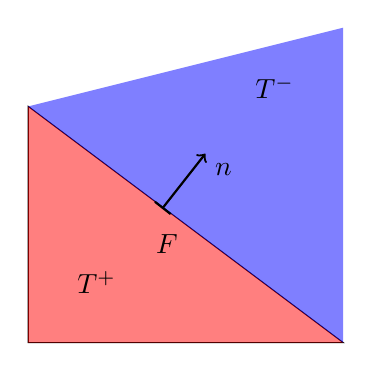
\begin{tikzpicture}[scale=1]
\coordinate (A) at (0,0);
\coordinate (C) at (0,3);
\coordinate (B) at (4,0);
\coordinate (D) at (4,4);
\coordinate (Tm) at (3.5,3.5);
\coordinate (Tp) at (0.5, 0.5);
\coordinate (e) at (1.5, 1.5);
\coordinate (start) at (1.7, 1.7);
\coordinate (end) at (2.25, 2.4);

\draw (A) -- (B) -- (C) -- cycle;
\fill[red, opacity=0.5] (A) -- (B) -- (C);
\fill[blue, opacity=0.5] (B) -- (C) -- (D);
\node[below left] at (Tm) {$T^{-} $ };
\node[above right] at (Tp) {$T^{+}$ };
\node[below right] at (e) {$F$ };

\draw [|->, thick] (start) -- (end);
% \node[above right] at (A) {A };
% \node[below right] at (B) {B};
% \node[above right] at (C) {C };
% \node[below right] at (D) {D};
\node[below right] at (end) {$n$};
\end{tikzpicture}
\caption{Facet $F \in \mathcal{F}_h $ shared by the triangles $T^{+}, T^{-} \in \mathcal{T}_{h} $ and the normal unit vector $n$.  }
    \label{fig:normal}
\end{figure}

A parameter which is useful is the maximum diameter $h$ of the set of triangles $\left\{ T \right\} $, which we to be defined such that,

\begin{equation}
\begin{split}
    h _{T} & = diam\left( T \right)   = \max_{x_1, x_{2} \in T} dist(x_{1}, x_{2}),  \\
    h_{min} & = \min_{T \in \mathcal{T} } h_{T}, \\
    h_{max} &= \max_{T \in \mathcal{T} }  h_{T} := h,
\end{split}
.\end{equation}




where the $diam( T )$ is the largest facet for a triangle $T$. We will also assume mesh conform i.e., if $T_{1} \neq T_{2 }$  and $T \cap T_{2} \neq \emptyset  $ , then they share either a vertex or a facet.
Let the chunkiness parameter $c_{T} := h_{T}/r_{T}$, where $r_{T}$  is the largest ball that be inscribed inside the element $T$.
We can then assume that the mesh is shape regular, i.e., that $c_{T}\le  c$ independent of $T$  and $h$. We may also assuming that
the mesh is quasi-uniform only if it holds that the mesh is shape regular and $h_{max} \le  c h_{min}$.

In this work will we compute norms on discontinuous elements, thus, it will be necessarry to define so-called broken mesh. Let us define $\mathcal{P} _{h}$ as an collection of geometric entities s.t. the norm and the inner product is defined as,
\[
 \| \cdot \|_{\mathcal{P}_{h}}^{2} = \sum_{P \in \mathcal{P} _{h}}^{} \| \cdot  \|_{ P }^{2  }, \quad \text{ and } \quad
 (\cdot ,\cdot )_{\mathcal{P}
_{h}}^{} = \sum_{P \in \mathcal{P} _{h}}^{} (\cdot ,\cdot )_{ P }^{  } .
\]

\newpage
\section{Unfitted cut discontinuous Galerkin method for the Poisson problem}%
\label{sec:elliptic}

\subsection{Poisson problem}%
\label{sub:possion_problem}
We will first consider the continuous Poisson problem. Let $f \in H^1( \Omega ) $ and $g \in H^{\frac{1}{2}}( \Gamma ) $ and $\Omega  \in \mathbb{R} ^{d}$ . We then define the strong formulation of the Possion problem to be \[
\begin{split}
    -\Delta u &= f \quad  \text{in }\Omega  \\
     u &= g  \quad \text{on } \Gamma    \\
\end{split} .
\]
Let us define the Hilbert spaces $V=H^{1}( \Omega ) $,   $V_{g} = \left\{ v \in H^{1}( \Omega ): v \mid _{\Gamma } = g \right\} $, the bilinear form $a: V \times V  \to \mathbb{R}  $ and the linear form $l: V'\to \mathbb{R}  $ s.t. \[
a( u,v) = ( \nabla u, \nabla v) _{\Omega }, \quad l( v) = (f,v)_{\Omega }.
\]
We say the weak formulation is to find a $u \in V_{g}$ so this equation holds  \[
a( u,v) = l( v), \quad  \forall v \in V
\]
\subsection{CutFEM }%
\label{sub:cutfem}


One of the key element to unfitted methods is that is relying on a background mesh. We denote the shape-regular and background mesh, $\widetilde{\mathcal{T}}_{h} $, to be a collection of $d$-dimensional simplices, $\left\{ T \right\} $, covering some closed domain
$\overline{\Omega } \subset \mathbb{R} ^{d} $.












